\chapter{PathBench} \label{Simulation Platform}

PathBench is a motion planning platform used to develop, assess, compare and visualise the performance and behaviour of the discussed algorithms. The platform is split into four main components: \textbf{Simulator}, \textbf{Generator}, \textbf{Trainer} and \textbf{Analyzer} joined by the infrastructure section. Additionally, the platform provides a \textit{ROS} real-time extension for interacting with a real-world robot through PathBench (See Figure \ref{fig: sim_platform}). The full architecture can be seen in Figure \ref{fig:sim_architecture}. 

% the platform provides a \textit{ROS} real-time extension which integrates the \textit{gmapping} \textit{ROS} package (SLAM scan) into a dedicated internal map environment (\textbf{RosMap}) controlled by a master node (\textbf{Ros})

\textbf{Notation.} We will use \textit{italic font} for libraries, \textbf{bold font} for classes and \texttt{typewriter font} for code snippets/file names/functions/variables. For types, we use the \textit{python} type hinting system (e.g. a list of integers is defined as \texttt{List[int]}).

% \todo{Mention ROS extension and add ROS components in high overview}

% The \textit{ROS} section provides compatibility with the \textit{ROS} library by integrating the \textit{gmapping} package (SLAM scan) into an internal map environment (\textbf{RosMap}). The \textbf{Ros} component represents the master node which controls the interactions between the robot and PathBench. 

\begin{figure}[h!]
    \centering
    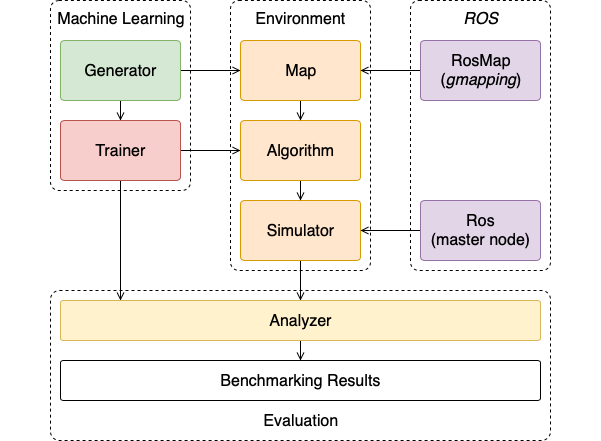
\includegraphics[scale=0.5]{images/sim_high_overview.png}
    \caption{PathBench structure high-overview. Arrows represent information flow/usage ($A \xleftarrow{gets/uses} B$). The Machine Learning section is responsible for training dataset generation and model training. The Environment section controls the interaction between the agent and the map, and supplies graphical visualisation. The \textit{ROS} section provides support for real-time interaction with a real physical robot. The Evaluation section provides benchmarking methods for algorithm assessment}
    \label{fig: sim_platform}
\end{figure}

\textbf{Infrastructure.} This component is responsible for linking all other components and provide general service libraries and utilities (for a comprehensive explanation of the infrastructure sub-components, please refer to Appendix \ref{sec: infra}).

\pagebreak

\textbf{Simulator.} This section is responsible for environment interactions and algorithm visualisation. It provides custom collision detection systems and a graphics framework for rendering the internal state of the algorithms.

\textbf{Generator.} This section is responsible for generating and labelling the training data used to train the Machine Learning models.

\textbf{Trainer.} This section is a class wrapper over the third party Machine Learning libraries. It provides a generic training pipeline based on the holdout method and standardised access to the training data.

\textbf{Analyzer.} The final section manages the statistical measures used in the practical assessment of the algorithms. Custom metrics can be defined as well as graphical displays for visual interpretations.

% the platform provides a \textit{ROS} real-time extension which integrates the \textit{gmapping} \textit{ROS} package (SLAM scan) into a dedicated internal map environment (\textbf{RosMap}) controlled by a master node (\textbf{Ros})

% The \textit{ROS} section provides compatibility with the \textit{ROS} library by integrating the \textit{gmapping} package (SLAM scan) into an internal map environment (\textbf{RosMap}). The \textbf{Ros} component represents the master node which controls the interactions between the robot and PathBench. 

\textbf{ROS Real-time Extension.} The extension provides real-time support for visualisation, coordination and interaction with a physical robot. The extension is split into two main components: \textbf{RosMap} (integrates the \textit{gmapping} \textit{ROS} package (SLAM scan) into a dedicated internal map environment) and \textbf{Ros (master node)}. We explain the \textbf{Ros (master node)} architecture and functionality in Section \ref{sec: robotexp} (\hyperref[sec: robotexp]{Path Planning on Real-world Robot}) in which we evaluate the performance of the proposed solution on a real robot.

\section{Comparison with other motion planner platforms}

Currently, there are a variety of standardised libraries which contain at least two of the mentioned sections (\textbf{Simulator} and \textbf{Analyzer}) such as: \textit{ROS} \cite{Quigley09}, \textit{OMPL} \cite{sucan2012the_open_motion_planning_library}, \textit{MoveIt} \cite{moveit} (has benchmarking capabilities \cite{moll2015benchmarking}).

\textbf{ROS.} The Robot Operating System (ROS) is a platform which contains various simulation environments (including 2D and 3D) for different types of robots: ground robots with different degrees of freedom constraints, flying robots (drones) and manipulator robots (arm robots which interact with different objects). It represents the standard library in robotics for simulation and development.

\textbf{OMPL.} The Open Motion Planning Library (OMPL) is a standalone library which focuses on motion planning exclusively. It is more lightweight than ROS and has reduced capabilities (there is no collision detection). The library of available path planners is limited to sampling-based planners such as RRT or PRM (probabilistic road maps), but there is a variety of optimised implementation for each type of planner.

\textbf{MoveIt.} Combines both ROS and OMPL to create a high-level implementation for cleaner and faster development of new algorithms. It has more capabilities than ROS and OMPL and includes custom benchmarking techniques \cite{moll2015benchmarking}.

\textbf{PathBench (our platform).} Our implementation offers a more abstract overview of the environment and is extremely lightweight compared to the mentioned libraries. We include both a simulation environment (\textbf{Simulator}) and benchmarking techniques (\textbf{Analyser}), but we also include a generator for creating synthetic datasets for Machine Learning applications (\textbf{Generator}) and a ML training pipeline (\textbf{Trainer}) for generic ML models. The \textbf{Analyser} is quite involved and extensible, but the \textbf{Simulator} has limited capabilities in both rendering and environment interaction compared to the other libraries. The main motivation of using our platform and not the existing standardised libraries is that the platform was build to be used in an ideal research environment. Since, we use ML methods, the focus was set on the path generation and not the interaction between the environment and the agent. However, we do provide a clean API interface for the algorithms which makes them portable to the standardised libraries. Moreover, we provide a \textit{ROS} real-time extension which converts the internal map move action into network messages (velocity control commands) using the \textit{ROS} publisher-subscriber APIs (See Table \ref{tab: plat_comparison} for platform comparison).

%\todo{SAJAD: A table showing features (support for ML, etc) vs platform (ROS, OMPLS, etc) would be the best fit for here.}

\begin{table}[h!]
    \footnotesize
    \centerfloat
    \begin{tabular}{|c|M{1.9cm}|M{2cm}|M{1.4cm}|M{1.9cm}|M{1.2cm}|M{1.8cm}|}
         \hline
         \textbf{Platform} & \textbf{Visualisation} & \textbf{Benchmarking} & \textbf{Machine Learning Support} & \textbf{Development Efficiency} & \textbf{Robot Variety} & \textbf{Environment Complexity and Interaction} \\
         \hline
         \textbf{ROS} & \checkmark & \xmark & \xmark & \textbf{Reduced} & \textbf{High} & \textbf{High} \\
         \hline
         \textbf{OMPL} & \checkmark & \xmark & \xmark & \textbf{High} & \textbf{Reduced} & \textbf{Reduced} \\
         \hline
         \textbf{MoveIt} & \checkmark & \checkmark & \xmark & \textbf{Moderate} & \textbf{High} & \textbf{High} \\
         \hline
         \textbf{PathBench} & \checkmark & \checkmark & \checkmark & \textbf{High} & \textbf{Reduced} & \textbf{Reduced} \\
         \hline
    \end{tabular}
    \caption{Platform capabilities comparison chart}
    \label{tab: plat_comparison}
\end{table}

\begin{figure}[h!]
    \centerfloat
    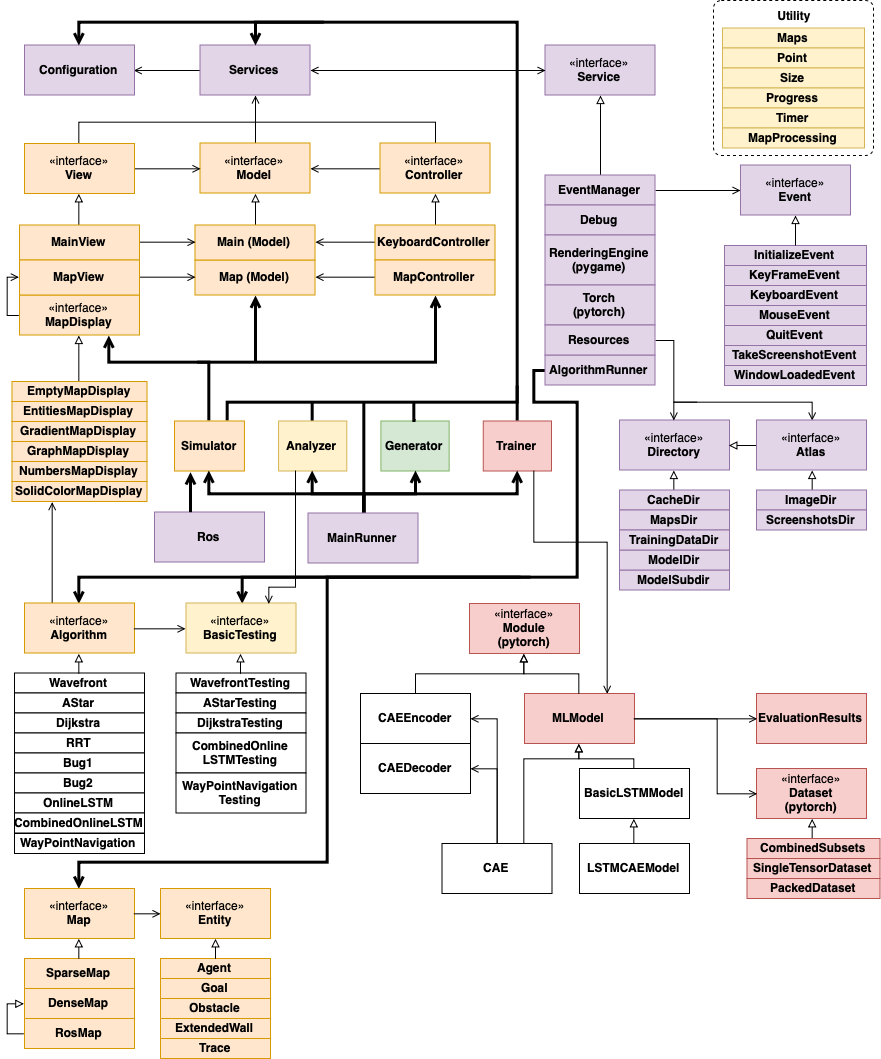
\includegraphics[scale=0.46]{images/simulator_architecture.png}
    \caption{Full platform architecture overview. Arrows with full head represent dependency ($A \xrightarrow{depends\, on/uses} B$) and arrows with hollow head represent inheritance ($A \xrightarrow{inherits\,from} B$). Colours are mapped as follows: purple is infrastructure, orange is simulator, green is generator, red is trainer, yellow is utility/analyser and white is extension}
    \label{fig:sim_architecture}
\end{figure}

\section{Implementation}

Before coding the platform, we have investigated a series of libraries and programming languages and we have decided to write it in \textit{python ver. 3.7.3}, use \textit{pytorch} \cite{paszke2017automatic} for machine learning and \textit{pygame} \cite{pygame} for rendering.

The choice of programming language was straightforward as \textit{python} is the standard in ML and research applications. Moreover, a lot of open source ML libraries are available such as \textit{tensorflow} \cite{tensorflow2015_whitepaper} and \textit{pytorch} which are used both in production software and researching.

For the ML library, we have chosen \textit{pytorch} over \textit{tensorflow}, because \textit{pytorch} was developed with the intent of it being used in research. \textit{tensorflow} is a mature ML library which has extensive community support, and it is used by major companies in production software, but, unlike \textit{pytorch}, it is quite hard to debug, due to the design of the computational graphs. In \textit{tensorflow}, you have to compile the model and use special session variables, while \textit{pytorch} offers the possibility of dynamically changing the computational graphs, which allows the user to debug more easily. This feature is most useful when dealing with RNNs with variable size inputs (in our case the LSTM) \cite{tensorflow_vs_pytorch}.

The simulator was build using the rendering library \textit{pygame}. The other choices included \textit{pyglet} \cite{pyglet} and \textit{Unity 3D} \cite{bartneck2015robot}. \textit{pyglet} is an advanced rendering engine which is based on \textit{OpenGL} \cite{opengl}, but due to the fact that we do not have graphics intensive requirements, a lightweight library such as \textit{pygame} is a better option. Moreover, \textit{pygame} provides useful rendering helper functions which do not require prior knowledge about \textit{OpenGL}, thus making development faster.

\textit{Unity 3D} was considered as an alternative to \textit{pygame} as it provides an additional physics engine which has collision detection and ray casting. Both features were needed in later development stages and had to be manually implemented. The main downside to choosing \textit{Unity 3D} was that we could not use \textit{pytorch} anymore, because \textit{Unity 3D} uses \textit{C\#} as the core programming language. There were multiple solutions to this issue: use \textit{IronPython}\footnote{\textit{IronPython} is a library which provides a \textit{python2} session wrapper that can be directly used in \textit{C\#} code} \cite{foord2009ironpython}, use the \textit{C\#} ML wrappers or create a ML server. However, none of them had a good trade-off to make the switch. Moreover, all solutions required different communication protocols which could have severely affected the performance of the path planners.

\section{Simulator}

The \textbf{Simulator} is both a visualiser tool and an engine for developing \textbf{Algorithm}s (See Figure \ref{fig: sim}). It supports animations and custom \textbf{MapDisplay} components which render the \textbf{Algorithm}'s internal data. Table \ref{tab: sim_commands} from Appendix \ref{sec: app_env} provides a list of user commands which control the simulator during run-time.

A \textbf{Map} contains different entities such as the \textbf{Agent}, \textbf{Goal} and \textbf{Obstacle}s, and provides a clean interface that defines the movement and interaction between them. Therefore, a \textbf{Map} can be extended to support various environments. The downside to this features is that each map has to implement its own physics engine or use a third party one (such as the \textit{pymunk} physics engine \cite{pymunk} or \textit{OpenAI Gym} \cite{OpenAI_Gym}). The current implementation supports three 2D maps: \textbf{DenseMap}, \textbf{SparseMap} and \textbf{RosMap}. 

The \textbf{DenseMap} stores entities in a grid format in order to reduce the time complexity of the APIs (i.e. collision detection, ray casting and line drawing). Collision detection is $\mathcal{O}(1)$, and most operations such as ray casting and line drawing are trivial to implement. When the agent has a radius attached to it, the obstacles are inflated by creating \textbf{ExtendedWall} objects around the obstacle boundary (the method is similar to the repulsion function from Potential Fields; time complexity is $\mathcal{O}(xo)$, where $x$ is the inflation rate and $o$ is the average obstacle size). The agent can overlap the \textbf{ExtendedWall} obstacles as long as the \textbf{ExtendedWall} obstacles do not contain its centre. 

Unlike the \textbf{DenseMap}, the \textbf{SparseMap} stores all entities in a list similar to \textit{Unity 3D}. It does not need obstacle inflation, and it has fast collision detection as only circles are used for each entity (circle collision is $\mathcal{O}(1)$), but it does not implement a pairwise checking algorithm (such as pairwise pruning or sweep and prune) and, thus, the complexity of the whole collision detection system becomes $\mathcal{O}(n^2)$ as all pairs of entities are checked. Thus, the \textbf{SparseMap} is mostly used to create user-defined maps which are then converted to a \textbf{DenseMap}.

% the platform provides a \textit{ROS} real-time extension which integrates the \textit{gmapping} \textit{ROS} package (SLAM scan) into a dedicated internal map environment (\textbf{RosMap}) controlled by a master node (\textbf{Ros})

% The \textit{ROS} section provides compatibility with the \textit{ROS} library by integrating the \textit{gmapping} package (SLAM scan) into an internal map environment (\textbf{RosMap}). The \textbf{Ros} component represents the master node which controls the interactions between the robot and PathBench.

%\todo{Talk about RosMap}
The \textbf{RosMap} extends the \textbf{DenseMap} to integrate the \textit{gmapping} \textit{ROS} package (SLAM scan) by converting the SLAM output image into an internal map environment. Because we extend the \textbf{DenseMap} component, we inherit the collision detection system and all additional functionality from it. The \textbf{RosMap} environment has support for live updates, meaning that algorithms can query an updated view by running a SLAM scan. The map uses simple callback functions to make SLAM update requests and convert movement actions into network messages using the \textit{ROS} publisher-subscriber communication system.

For all maps, movement is allowed in eight directions: horizontal, vertical and diagonal (movement cost is based on the Euclidean distance: horizontal/vertical 1 and diagonal $\sqrt{2}$). It should be noted that, because we are simulating the map environment, we need the full map information for \textbf{SparseMap} and \textbf{DenseMap}. However, because we provide a \textbf{Map} interface, we can define custom maps (such as \textbf{RosMap}) that restrict the agent information access (e.g. in the real world, the robot usually does not has access to the full information of the environment).

Additionally, the \textbf{Simulator} provides animations that are achieved through key frames and synchronisation primitives (the process is described in Appendix \ref{sec: infra}).

\begin{figure}[h]
  \centering
  \begin{subfigure}[b]{0.2\linewidth}
    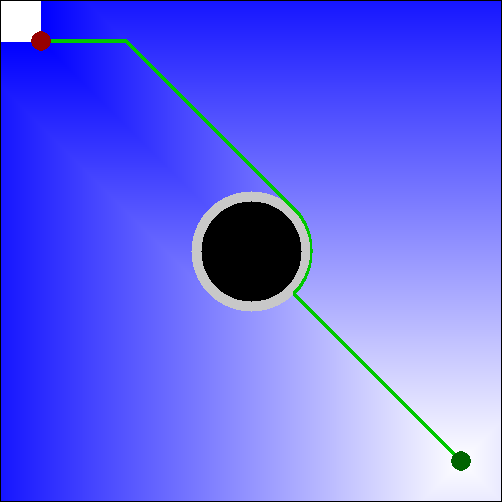
\includegraphics[width=\linewidth]{images/screenshot_43.png}
     \caption{Wave-front planner (\ref{sec: wave-front})}
  \end{subfigure}
  \hfill
  \begin{subfigure}[b]{0.2\linewidth}
    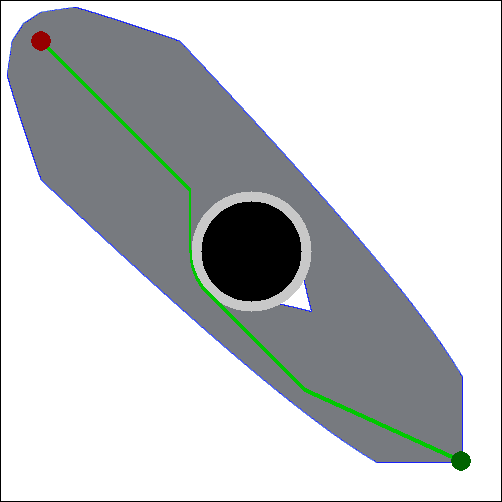
\includegraphics[width=\linewidth]{images/screenshot_44.png}
    \caption{A* (\ref{sec:a_star}) \newline}
  \end{subfigure}
  \hfill
  \begin{subfigure}[b]{0.2\linewidth}
    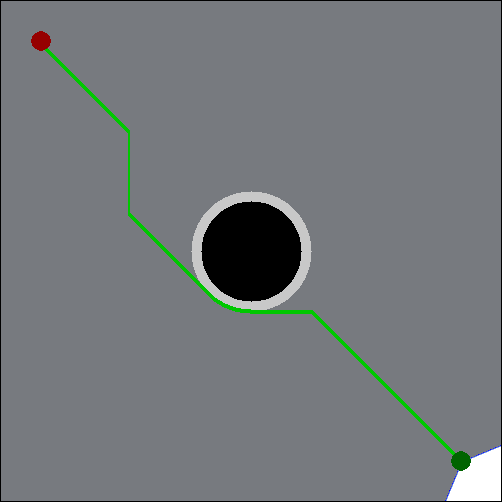
\includegraphics[width=\linewidth]{images/screenshot_46.png}
     \caption{Dijkstra (\ref{sec: dijkstra}) \newline}
  \end{subfigure}
  \hfill
  \begin{subfigure}[b]{0.2\linewidth}
    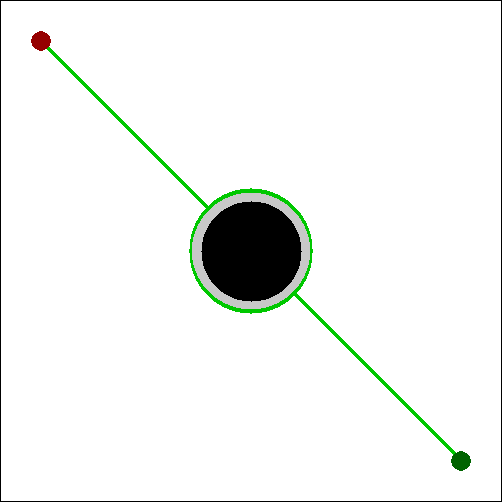
\includegraphics[width=\linewidth]{images/screenshot_47.png}
     \caption{Bug 1 (\ref{sec: bug1}) \newline}
  \end{subfigure}
  \newline
  \begin{subfigure}[b]{0.2\linewidth}
    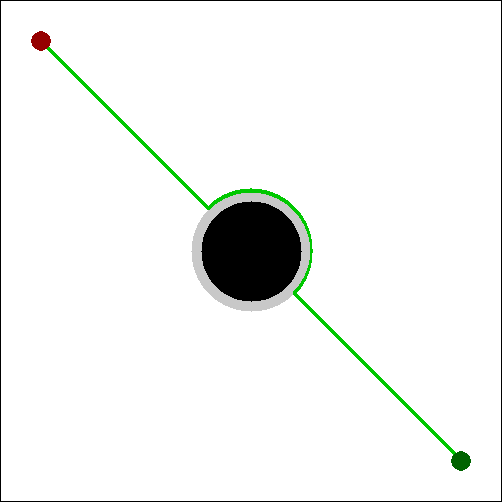
\includegraphics[width=\linewidth]{images/screenshot_48.png}
     \caption{Bug 2 (\ref{sec: bug2}) \newline}
  \end{subfigure}
  \hfill
  \begin{subfigure}[b]{0.2\linewidth}
    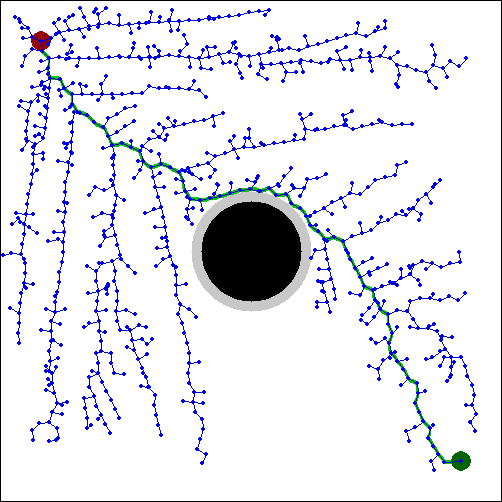
\includegraphics[width=\linewidth]{images/screenshot_49.png}
    \caption{RRT (\ref{sec: RRT}) \newline}
  \end{subfigure}
  \hfill
  \begin{subfigure}[b]{0.2\linewidth}
    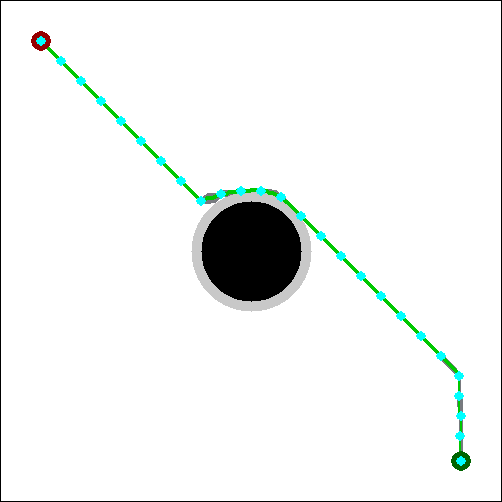
\includegraphics[width=\linewidth]{images/screenshot_51.png}
     \caption{Global Way-point LSTM Planner (\ref{sec: way point nav})}
  \end{subfigure}
  \hfill
  \begin{subfigure}[b]{0.2\linewidth}
    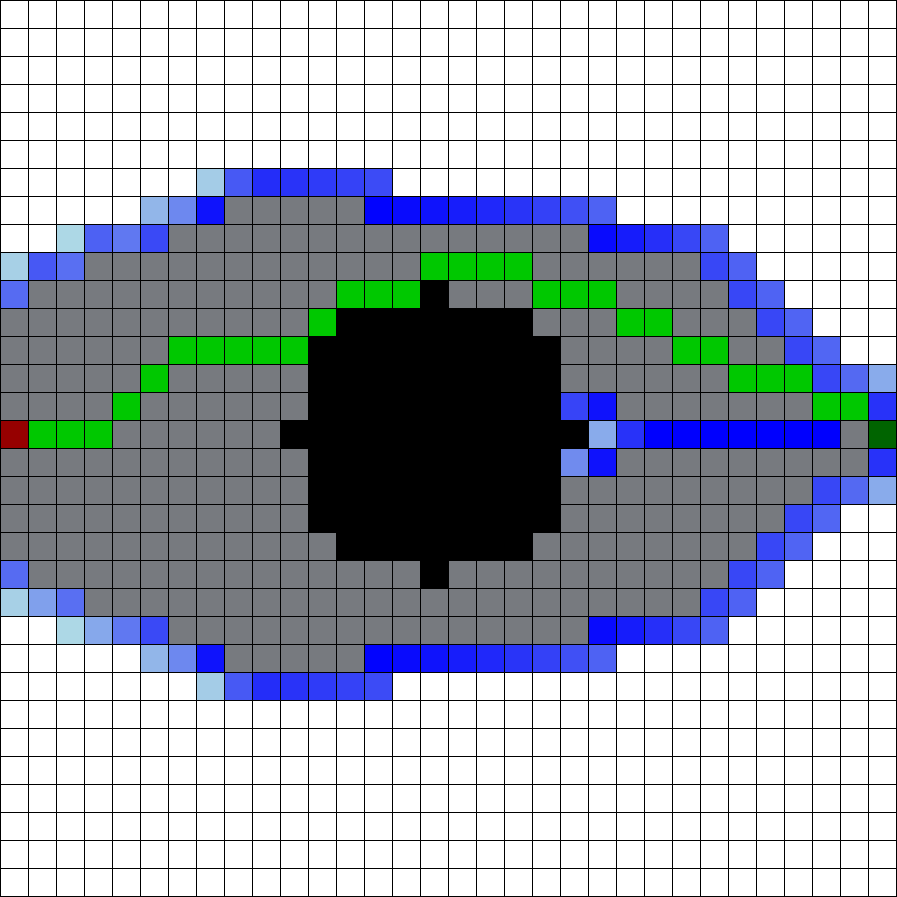
\includegraphics[width=\linewidth]{images/screenshot_50.png}
    \caption{A* (\ref{sec:a_star}) on a grid display}
  \end{subfigure}
  \caption{Different planners run on the same map (except Sub-figure (h)). The red entity is the agent, the green entity is the goal, light green entities are traces, black/light grey entities are obstacles and everything else is custom display information (e.g. in Sub-figure (b) dark grey represents search space)}
  \label{fig: sim}
\end{figure}

\pagebreak

\section{Generator} \label{sec: generator}

The \textbf{Generator} can execute five actions: conversion from image to map, map generation, map labelling, map augmentation and map modification.

\textbf{Conversion.} An image can be converted into an internal \textbf{Map} and saved into the maps directory from \textbf{Resources}. The image can be a software drawn image or Simultaneous Localization and Mapping (SLAM) image \cite{dissanayake2001solution} output from a real robot, as long as it follows the conventions imposed by the image converter: an agent represented by a true red circle has to be present, a goal represented by a true green circle has to be present and the obstacles need to be in the grey-black colour range (See Figure \ref{fig: converted map}).

\begin{figure}[h]
  \centering
  \begin{subfigure}[b]{0.3\linewidth}
    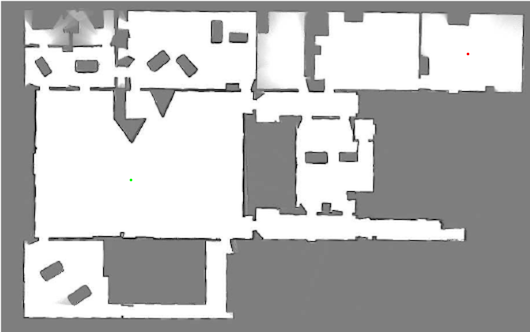
\includegraphics[width=\linewidth]{images/map10.png}
     \caption{Original SLAM Image}
  \end{subfigure}
  \hspace{1.5cm}
  \begin{subfigure}[b]{0.3\linewidth}
    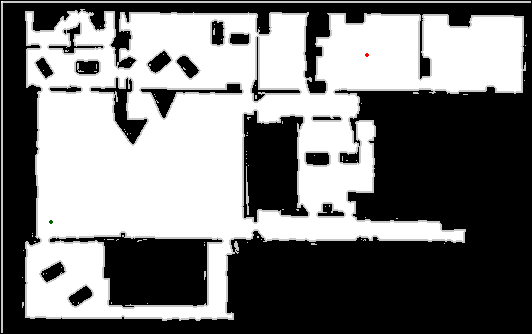
\includegraphics[width=\linewidth]{images/screenshot_108.png}
     \caption{Converted \textbf{Map}}
  \end{subfigure}
  \caption{Example of the conversion process from the \textbf{Generator}}
  \label{fig: converted map}
\end{figure}

%\todo{Sajad: do you ever refer to Fig 4.2-h? it seeme like a  repetition of 4.3-b.}
% The repetion is used to hilight that the simulator has a grid display as well, even if it is the same algorithm

%\todo{Sajad: It is very common to use 'Figure X' instead of 'figure X' and 'Algorithm Y' instead of 'Algorithm Y' and 'Table Z' instead of 'table Z' when you want to refer a figure, alg, or table in the text.}

% comment messes latex will put at top

\textbf{Generation.} The generation procedure accepts as input, different hyper-parameters such as the type of generated map, number of generated maps, obstacle fill rate range, number of obstacle range, minimum room size range and maximum room size range, which define the structure of the maps. When a range is given as input, the generator picks a random number between the range and feeds it into the associated map type generator. Currently, the generator can produce three types of maps: uniform random fill map (See Algorithm \ref{alg: Uniform random fill generator}), block map (See Algorithm \ref{alg: Block map generator}) and house map (See Algorithm \ref{alg: House generator}) (See Figure \ref{fig: generated maps}) and it can easily be extended to support different synthetic maps such as mazes and cave generation using cellular automata. All generated maps are placed into a new \textbf{Atlas} directory which is a custom directory that saves files using the index number. It keeps track of the next available index, and thus, when a new file is saved, it is "appended" to it. \textbf{Atlas} directories are used for easier indexing operations such as index loading and index saving (the file system service is described in Appendix \ref{sec: infra}).

\begin{figure}[h!]
  \centering
  \begin{subfigure}[b]{0.3\linewidth}
    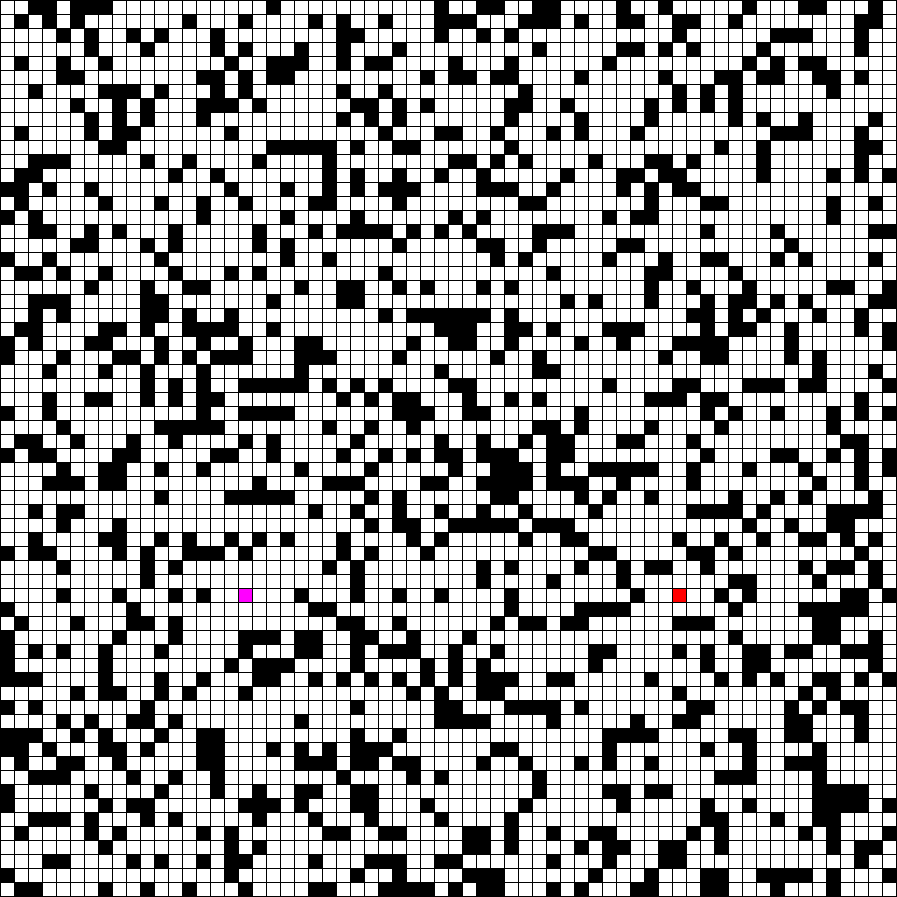
\includegraphics[width=\linewidth]{images/screenshot_52.png}
     \caption{Uniform random fill (64x64 dimension, [0.1, 0.3] obstacle fill rate range)\newline}
  \end{subfigure}
  \hfill
  \begin{subfigure}[b]{0.3\linewidth}
    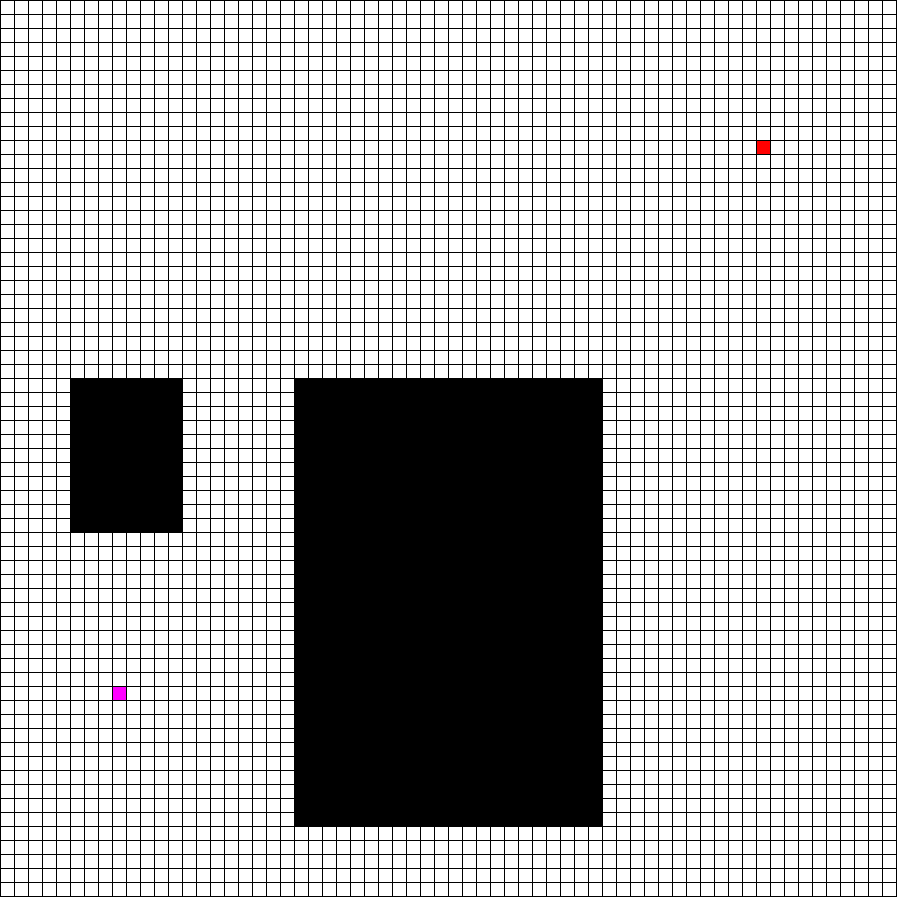
\includegraphics[width=\linewidth]{images/screenshot_54.png}
     \caption{Block map (64x64 dimension, [0.1, 0.3] obstacle fill rate range, [1, 6] number of obstacles range)}
  \end{subfigure}
  \hfill
  \begin{subfigure}[b]{0.3\linewidth}
    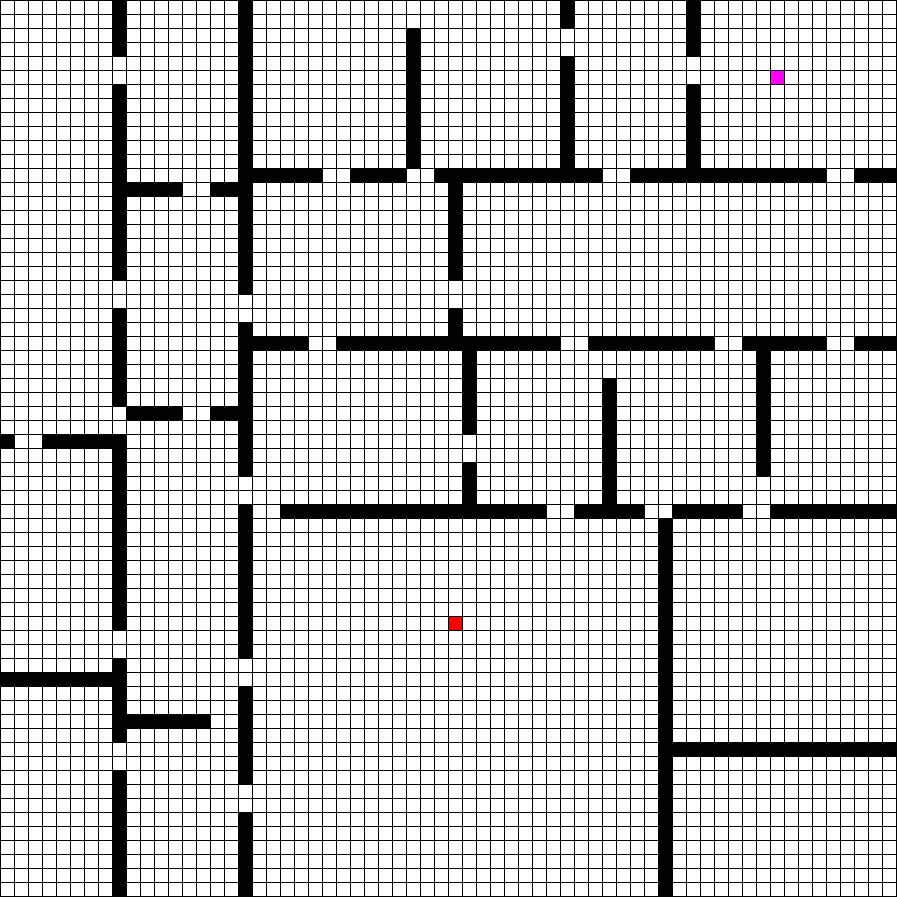
\includegraphics[width=\linewidth]{images/screenshot_53.png}
     \caption{House (64x64 dimension, [8, 15] minimum room size range, [35, 45] maximum room size range)}
  \end{subfigure}
  \caption{The current generated maps are: (a) Uniform random fill (10000 samples), (b) Block map (10000 samples), (c) House atlas (10000 samples). We will use magenta colour for the goal for all generated maps as the dark green goal is quite hard to spot}
  \label{fig: generated maps}
\end{figure}

\begin{algorithm}[!htb]
\caption{Uniform random fill generator}
\label{alg: Uniform random fill generator}
\begin{algorithmic}[1]
\Procedure{Generate-Uniform-Random-Fill-Map}{$dimension$, $obstacle\_fill\_rate$}
    \State Initialise empty $map$ of dimension $dimension$
    \State $fill \gets obstacle\_fill\_rate * dimension.width * dimension.height$
    \State $nr\_of\_obstacles \gets 0$
    \State
    \While {$nr\_of\_obstacles < fill$}
        \State $obstacle\_position \gets$ random position within $dimension$
        \If {$obstacle\_position$ is free on $map$}
            \State place unity obstacle at $obstacle\_position$ on $map$
            \State increment $nr\_of\_obstacles$ 
        \EndIf
    \EndWhile
    \State
    \State place agent and goal at random free positions on $map$
    \State \Return $map$
\EndProcedure
\end{algorithmic}
\end{algorithm}

\begin{algorithm}[!htb]
\caption{Block map generator}
\label{alg: Block map generator}
\begin{algorithmic}[1]
\Procedure{Generate-Block-Map}{$dimension$, $obstacle\_fill\_rate$, $nr\_of\_obstacles$}
    \State Initialise empty $map$ of dimension $dimension$
    \State $fill \gets obstacle\_fill\_rate * dimension.width * dimension.height$
    \State
    \For {$i$ in [0, $nr\_of\_obstacles$)}
        \State $next\_obst\_fill \gets$ random value from $fill$
        \While {can't place block}
            \State $first\_side \gets$ random value from $next\_obst\_fill$
            \State $second\_side \gets$ $next\_obst\_fill$ / $first\_side$
            \State try to place block of dimension ($first\_side$, $second\_side$) on random position (blocks may overlap)
        \EndWhile
        \State 
        \State $fill \gets fill - next\_obst\_fill$
    \EndFor
    \State
    \State place agent and goal at random free positions on $map$
    \State \Return $map$
\EndProcedure
\end{algorithmic}
\end{algorithm}

\begin{algorithm}[!htb]
\caption{House generator}
\label{alg: House generator}
\begin{algorithmic}[1]

\Procedure{Subdivide}{$top\_left\_corner, dimension$}
    \If{can't split anymore due to $min\_room\_size$}
        \State place a room at $top\_left\_corner$ with dimension $dimension$
    \EndIf
    \State
    \If{$dimension \leq max\_room\_size$}
        \State 50\% change to place a room at $top\_left\_corner$ with dimension $dimension$
    \EndIf
    \State
    \State random pick vertical or horizontal
    \State random split vertical/horizontal into 2 blocks: $first\_block$, $second\_block$
    \State
    \State $\textit{Subdivide}(first\_block\_top\_left\_corner, first\_block\_dimension)$
    \State $\textit{Subdivide}(second\_block\_top\_left\_corner, second\_block\_dimension)$
\EndProcedure

\Procedure{Generate-House-Map}{$dimension$, $min\_room\_size$, $max\_room\_size$}
    \State Initialise empty $map$ of dimension $dimension$
    \State
    \State $\textit{Subdivide}((-1, -1), dimension + 1)$
    \For{\ \textbf{each} $room$}
        \State get $room$ walls and add doors with probability 25\% (max 1 door per wall)
    \EndFor
    \State
    \State place agent and goal at random free positions on $map$
    \State \Return $map$
\EndProcedure
\end{algorithmic}
\end{algorithm}

\clearpage

\textbf{Labelling.} The labelling procedure takes a map \textbf{Atlas} and converts it into training data by picking only the specified features and labels. The training data is then saved as a \texttt{.pickle} file with name format as \texttt{training\_\{atlas name\}\_\{number of samples\}}. The structure of the training data is based on normal \textit{python} objects (\texttt{List[Dict[str, Any]]}) for quick inspection and analysis. Features/labels are picked by using the \textbf{MapProcessing} component (See Table \ref{tab: gen_label_list} for feature reference). A* is used as ground truth for feature/label generation. All features/labels can be saved as a variable sequence (needed for LSTM) or single global input (needed for auto-encoder).

\begin{table}[h!]
    \centerfloat
    \begin{tabular}{|M{5cm}|M{9cm}|}
        \hline
        \textbf{Feature/Label Key} &  \textbf{Description} \\
        \hline
        agent\_position & The current agent position \\
        \hline
        direction\_to\_goal & The current direction from the agent to the goal \\
        \hline
        direction\_to\_goal\_normalized & The normalised direction from the agent to the goal \\
        \hline
        distance\_to\_goal & The current Euclidean distance from the agent to the goal\\
        \hline
        distance\_to\_goal\_normalized(n) & The current normalised Euclidean distance from the agent to the goal (normalisation is done by clamping the output between [0, n))\\
        \hline
        raycast\_8 & The current distance from agent to obstacles on all eight directions (vertical, horizontal, diagonal) \\
        \hline
        raycast\_8\_normalized(n) & The current normalised distance from agent to obstacles on all eight directions (vertical, horizontal, diagonal) (normalisation is done by clamping the output between [0, n)) \\
        \hline
        agent\_goal\_angle & The current angle defined by the line segment from the agent to the goal (code $torch.atan2(v.y, v.x)$, where $v$ is the line segment)\\
        \hline
        valid\_moves & The current 0-1 tensor which describes in which direction (vertical, horizontal, diagonal) is agent movement available (1 is available) \\
        \hline
        global\_map & The current whole map obstacles given as a normalised 0-1 tensor (1 is obstacle)\\
        \hline
        local\_map & Like global\_map, but it has $9\times9$ dimension and agent is centred \\
        \hline
        next\_position & The next move direction that the agent should take \\
        \hline
        next\_position\_index & The next action that the agent should take given as an index from 0 to 7 \\
        \hline
    \end{tabular}
    \caption{\textbf{Generator} list of features and labels. A* is used as ground truth for label annotation}
    \label{tab: gen_label_list}
\end{table}

\textbf{Augmentation.} The augmentation procedure takes an existing training data file and augments it with the specified extra features and labels. It is used to remove the need for re-generating a whole training set.

\textbf{Modification.} A custom lambda function which takes as input a \textbf{Map} and returns another \textbf{Map} can be defined to modify the underlining structure of the map (e.g. modify the agent position, the goal position, create doors, etc.).
\section{Trainer}

The training pipeline is composed of: data pre-processing, data splitting, training, evaluation, results display and pipeline end. All ML models must inherit from the \textbf{MLModel} class. The model is passed through the pipeline together with a configuration file (\texttt{Dict[str, Any]}) which describes the training process (See Table \ref{tab: pipeline_config} for general configuration hyper-parameters). Each model can define extensions for all pipeline sections and extra configuration parameters. 

\begin{table}[h!]
    \centerfloat
    \begin{tabular}{|M{3.2cm}|M{2.3cm}|M{3.3cm}|M{4.4cm}|}
         \hline
         \textbf{Key} & \textbf{Pipeline Section} & \textbf{Type} & \textbf{Description} \\
         \hline
         data\_features & Data Pre-processing & \texttt{List[str]} & Which sequential features should be picked from training data \\
         \hline
         data\_labels & Data Pre-processing & \texttt{List[str]} & Which sequential labels should be picked from training data \\
         \hline
         data\_single\_features & Data Pre-processing & \texttt{List[str]} & Which single features should be picked from training data \\
         \hline
         data\_single\_labels & Data Pre-processing & \texttt{List[str]} & Which single labels should be picked from training data \\
         \hline
         training\_data & Data Pre-processing & \texttt{List[str]} & Which training data files should be loaded and feature/label picked\\
         \hline
         validation\_ratio & Data Splitting & \texttt{float} & How much validation data should be reserved from data \\
         \hline
         test\_ratio & Data splitting & \texttt{float} & How much evaluation data should be reserved from data \\
         \hline
         epochs & Training & \texttt{int} & How many times should data be passed during training\\
         \hline
         batch\_size & Training & \texttt{int} & Defines the batch size for each epoch \\
         \hline
         loss & Training & \texttt{Callable[[Tensor, Tensor], Tensor]} & Describes the loss function: Arguments(model output, label), Returns(loss value) \\
         \hline
         optimizer & Training & \texttt{Callable[[MLModel], Optimizer]} & Describes the optimizer that should be used: Arguments(model itself), Returns(optimizer) \\
         \hline
         save\_name & Pipeline End & \texttt{str} & The model save name \\
         \hline
    \end{tabular}
    \caption{Training pipeline basic configuration (more algorithm-specific training configurations are provided in Chapter \ref {Evaluation} (\hyperref[Evaluation]{Evaluation}))}
    \label{tab: pipeline_config}
\end{table}

\textbf{Data Pre-processing.} Data is loaded from the specified training sets, and only the features and labels used throughout the model are picked from the training set and converted to a \textit{pytorch} \textbf{Dataset} (in total there can be four datasets: one feature sequence, one single feature tensor, one label sequence and one single label tensor). Sequential data is wrapped into a \textbf{PackedDataset} which sorts the input in reverse order of its sequence length (max length first, min length last). The data is packed into a \textit{pytorch} \textbf{PackedSequence} object using the \texttt{pack\_sequence} function from \textit{pytorch}. The \texttt{pack\_sequence} function only accepts sorted sequences (i.e. the input should be an upper triangular matrix) in order to increase the speed of an LSTM forward pass. The \textbf{PackedDataset} class saves the sequence itself, the lengths and the sorting permutation. If both sequence and single features are available the single feature tensor is sorted as well according to the permutation used in \textbf{PackedDataset} and wrapped into a \textbf{TensorDataset}. Both datasets are returned as a \textbf{CombinedSubsets} object. The resulting \textbf{Dataset} is cached, because data pre-processing takes a long time and consumes a lot of memory (for 30000 samples, over 16 GB of RAM are needed).

\textbf{Data Splitting.} The pre-processed data is shuffled and split into three categories: training, validation and testing (usually 60\%, 20\%, 20\%) according to the Holdout method. The \textbf{CombinedSubsets} object is used to couple the feature dataset and label dataset of the same category into a single dataset. Then, all data is wrapped into its \textbf{DataLoader} object with the same batch size as the training configuration (usually 50).

\textbf{Training.} The training process puts the model into training mode and takes the training \textbf{DataLoader} and validation \textbf{DataLoader} and feeds them through the model $n$ times, where $n$ is the number of specified epochs. The training mode allows the gradients to be updated and at each new epoch, the optimiser sets all gradients to 0. Each model has to extend a special \texttt{batch\_start} hook function which is called on each new batch. The \texttt{batch\_start} function is responsible for passing the data through the network and returning the loss result. The trainer takes the loss result and applies a backward pass by calling the \texttt{.backward()} method from the loss. Afterwards, the optimiser is stepped, and the weights of the model are updated. The statistics, such as the loss over time, for the training and validation sets are logged by two \textbf{EvaluationResults} objects (one for training and one for validation) which are returned to the pipeline. The \textbf{EvaluationResults} class contains several hook functions which are called through the training process at their appropriate times: \texttt{start}, \texttt{epoch\_start}, \texttt{epoch\_finish}, \texttt{batch\_start}, \texttt{batch\_finish}, \texttt{finish}. At each epoch end, the \textbf{EvaluationResults} object prints the latest results.

\textbf{Evaluation.} The evaluation process puts the model into evaluation mode and has a similar structure to the training process. The evaluation mode does not allow gradients to update. The testing dataset is passed only once through the model and an \textbf{EvaluationResults} object containing the final model statistics is returned to the pipeline.

\textbf{Results Display.} This procedure displays the final results from the three \textbf{EvaluationResults} objects (training, validation, testing) and final statistics such as the model loss are printed. The training and validation loss logs are displayed as a \textit{matplotlib} \cite{Hunter:2007} figure. This method can be easily extended to provide more insight into the network architecture (e.g. the \textbf{CAE} model displays a plot which contains the original image, the reconstructed version, the latent space snapshot and the resulting feature maps).

\textbf{Pipeline End.} At the end, the model is saved by serialising the model \texttt{.state\_dict()}, the model configuration, the plots from results display process and the full printing log into a \textbf{ModelSudir} under \textbf{ModelDir}. The save name is formated according to the following convention: \texttt{\{config save\_name\}\_\{config training\_data\}\_model}.

%\newpage
\section{Analyser}

The \textbf{Analyser} is used to assess and compare the performance of the path planners. This is achieved by making use of the \textbf{BasicTesting} component. When a new session is run through the \textbf{AlgorithmRunner}, if a \textbf{BasicTesting} component is attached to it, the session records a series of statistical measures depending on the type of testing (See Table \ref{tab: a_testing_tab}). The \textbf{BasicTesting} component is also linked to the simulator to enable visualisation testing. The key frame feature and synchronisation variable are tied to the \textbf{BasicTesting} component, which allows the user to enhance each key frame and define custom behaviour. Each \textbf{Algortihm} instance can create debugging views called \textbf{MapDisplay}s which can render custom information on the screen such as the the internal state of the \textbf{Algortihm} (e.g. Search Space, Total Fringe) (See Table \ref{tab: map_dsiplays}).

\begin{table}[h!]
    \centerfloat
    \begin{tabular}{|c|M{2.7cm}|M{8cm}|}
         \hline
         \textbf{Name} & \textbf{Supported Algorithms} & \textbf{Description} \\
         \hline
         Map & \texttt{All} & The actual map \\
         \hline
         Trace & \texttt{All} & The actual trace points \\
         \hline
         Map Obstacle Ratio & \texttt{All} & The percentage of obstacles from the map \\
         \hline
         Original Distance & \texttt{All} & The Euclidean distance from agent to goal at the beginning of the algorithm \\
         \hline
         Algorithm Type & \texttt{All} & The type of the algorithm that was run \\
         \hline
         Success Rate & \texttt{All} & The rate of success of finding a path from the agent to the goal \\
         \hline
         Steps & \texttt{All} & The total steps (movements) taken to reach the goal \\
         \hline
         Distance & \texttt{All} & The total distance taken to reach the goal. Steps is different from Distance as the diagonal movement cost is 1, but the diagonal movement cost is $\sqrt{2}$ \\
         \hline
         Time & \texttt{All} & The total time taken to reach the goal \\
         \hline
         Distance Left & \texttt{All} & In case of failure what is the Euclidean distance left from the agent to the goal \\
         \hline
         Search Space & \texttt{A*}, \texttt{Dijkstra} & The search space that was used to find the path (visited set without priority queue) \\
         \hline
         Total Fringe & \texttt{A*}, \texttt{Dijkstra} & The left priority queue size, after the goal was found \\
         \hline
         Total Search & \texttt{Wave-front}, \texttt{A*}, \texttt{Dijkstra} & Total Search = Search Space + Total Fringe \\
         \hline
    \end{tabular}
    \caption{\textbf{Analyser} general statistic measures (more algorithm-specific metrics are provided in Chapter \ref {Evaluation} (\hyperref[Evaluation]{Evaluation}))}
    \label{tab: a_testing_tab}
\end{table}

\begin{table}[h!]
    \centerfloat
    \begin{tabular}{|M{2cm}|M{2.7cm}|M{9.2cm}|}
         \hline
         \textbf{Display Name} & \textbf{Supported Algorithms} & \textbf{Description} \\
         \hline
         Map & \texttt{All} & Displays the map in two modes: grid, normal \\
         \hline
         Entities & \texttt{All} & Displays the map entities: clear tiles (white), agent (red), goal (dark green), obstacles (black), extensions (light grey), trace (light green) \\
         \hline
         Step Grid (gradient) & \texttt{Wave-front} & Displays the step grid (white-dark blue gradient, min is white, max is dark blue) \\
         \hline
         Step Grid (numbers) & \texttt{Wave-front} & Displays the actual numbers from the step grid (simulator has to be launched in grid display mode) \\
         \hline
         Search Space and Total Fringe & \texttt{A*}, \texttt{Dijkstra} & Displays the visited set (dark grey) and the priority queue (fringe) (light blue-dark blue gradient, the darker the blue, the higher the priority) \\
         \hline
         Graph & \texttt{RRT} & Displays the graph edges (blue lines) and graph nodes (blue circles) \\
         \hline
    \end{tabular}
    \caption{\textbf{Algorithm} information displays (more algorithm-specific information displays are provided in Chapter \ref {Evaluation} (\hyperref[Evaluation]{Evaluation}))}
    \label{tab: map_dsiplays}
\end{table}

Instead of manually running a \textbf{Simulator} instance to assess an \textbf{Algorithm}, the \textbf{Analyser} has an extensive algorithmic analysis procedure split into two parts: simple analysis and complex analysis. We also provide a training dataset analysis routine for inspecting the generated maps.

\textbf{Simple Analysis.} $n$ (usually 10) map samples are picked from each generated map type, and $m$ algorithms are assessed on them. The results are averaged and printed.

\textbf{Complex Analysis.} $n$ maps are selected (generated or hand-made), and all $m$ algorithms are run on each map $x$ (usually 50) times with random agent and goal positions. As in the simple analysis stage, the results are averaged and reported. In the end, all $n \times x$ results are averaged and reported.

\textbf{Training Dataset Analysis.} A training set analyser procedure is provided to inspect the training datasets by using the basic metrics defined in Table \ref{tab: a_testing_tab} (e.g. Original Distance, Success Rate, Map Obstacle Ratio).

All printing from the three sections is saved in log files in the \textbf{Resources} directory. In order to view and interpret the results in a friendlier format, the results are tabulated (a latex table generator helper function is used to transfer the results from the log to the report). 
